\documentclass[]{article}

%opening
\title{Automated Reading Comprehension Clustering}
\author{Charles Hathaway}

\usepackage[final]{pdfpages}
\usepackage{graphicx}
\usepackage[style=ieee,backend=bibtex]{biblatex}

\bibliography{biblo}

\begin{document}

\maketitle

\section{Executive Summary}

This project will focus on discussing and exploring the effectiveness of various language features when applied to clustering books based on reading comprehension level.
It will utilize previous works in the area, which although may not be perfectly applicable, have a somewhat obvious connection to the objective.
To test the features, we will attempt to generate 3 clusters from plain-text books freely available online; child-friendly, young adult, and adult books.

The timetable for this project is given at the end of the document.

\section{Goal}

The goals of this project are:
\begin{itemize}
	\item Exploration of existing reading comprehension features and clustering tools
	\item Testing of new and existing reading comprehension features
	\item Analysis of results and discussion
	\item Interface to allow others to utilize the tool
\end{itemize}

\section{Background and Motivation}

There are several systems currently used to classify books based on reading comprehension level, for numerous applications ranging from selecting books for classrooms, to measuring an individuals literacy skills for both medical (autism, dyslexia, etc.) and educational purposes.
The goal of this project is to enable a larger selection of books for these purposes by automated the system of clustering books by grade level, which is currently manually done at the cost of the publisher.

\section{System Architecture and Approach}

Following many other NLP applications, this project will utilize a pipeline approach.
This pipeline is laid out in figure \ref{flowchart}.
The design is further described in the box chart, displayed in figure \ref{boxchart}.

In order to accelerate development, the coding will primarily be done in Python.
The project will utilize various open source toolkits, including the NLTK, which provides a maximum entropy clustering framework.
This will allow me to spend more time focusing on selecting effective features, and less time remaking the wheel.

\section{Deliverables}

The deliverables of this project will have 3 key parts:
\begin{itemize}
	\item A technical report, detailing the results of key experiments and output of several configurations of the systems
	\item A command-line interface that allows the scanning and clustering of a multitude of books
	\item A web interface which outputs the cluster a particular uploaded books belongs to
\end{itemize}

\section{Required Resources}

The most important resources for this project is the books themselves.
To that end, Project Gutenberg will be mined to provide both the training and testing data sets.
They have an extensive list of childrens books, which we will use as the basis for the first clustering.
Ideally, we will end up with a clustering such that childrens book all fall below the average reading difficulty, at average - 1 standard deviation.
For the second clustering, we will determine it by picking a range in between the children books and the highest threshold; ideally in the range of average $\pm$ 1 standard deviation.
The last section, adult/advanced readers, will consist of books deemed more complicated than the average + 1 standard deviation.

It should be noted that the Project Gutenberg repository is large; upwards of 650GB.
Most books in the project have multiple translations, which contributes to the large size (in addition to multiple translations, they also have multiple format).
To make this project more achievable, we will limit ourselves to the fiction category; which has it's own subcategory, children's fiction.

Lastly, we need a toolkit which provides many resources to help calculate the clusters given our feature set.
For this purpose, we will use the Python Natural Language Toolkit (NLTK), which is a free and open source library intended for these types of application \cite{ref:evolution_of_jun}.

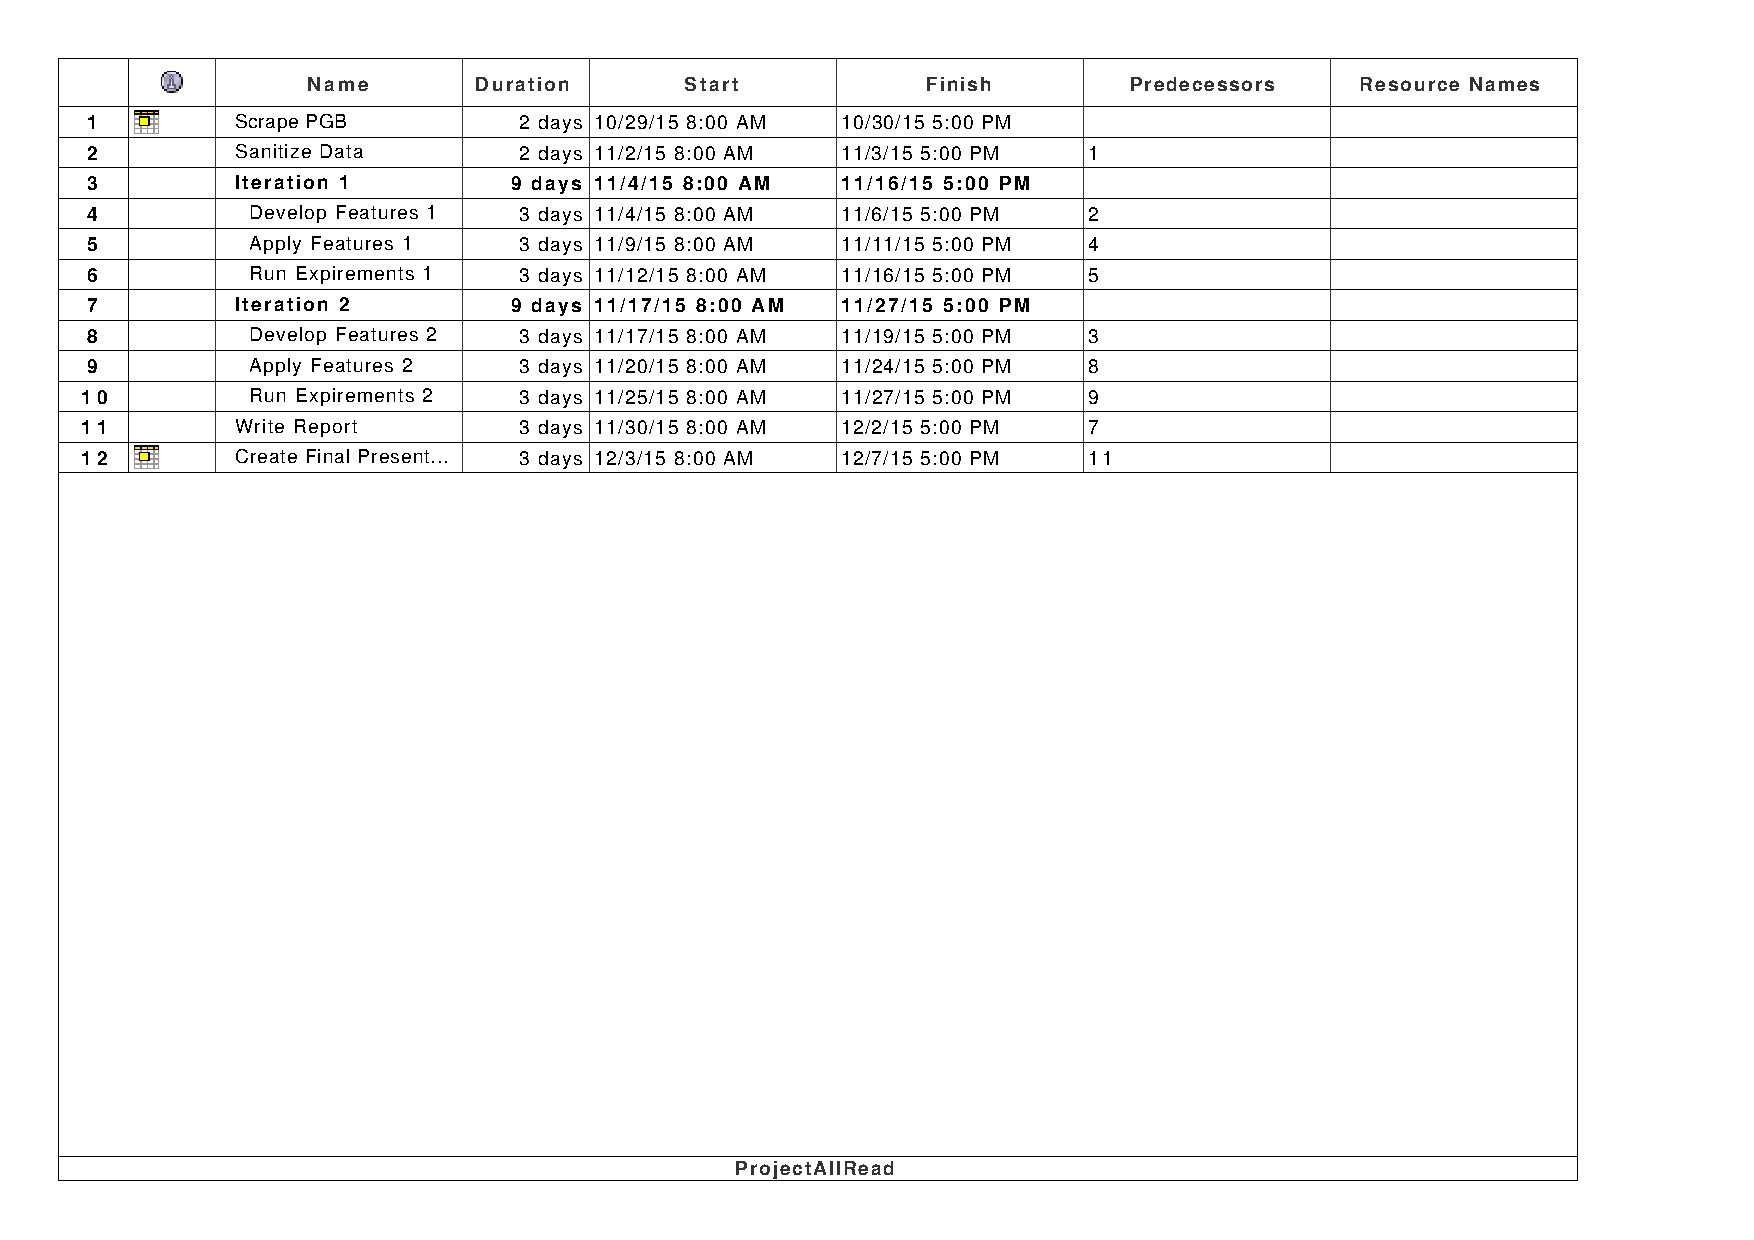
\includepdf[pages=1]{../ProjectAllRead.pdf}



\begin{figure}
	\label{flowchart}
	\caption{Flowchart indicating flow of information within system}
	\centering
	\makebox[\textwidth]{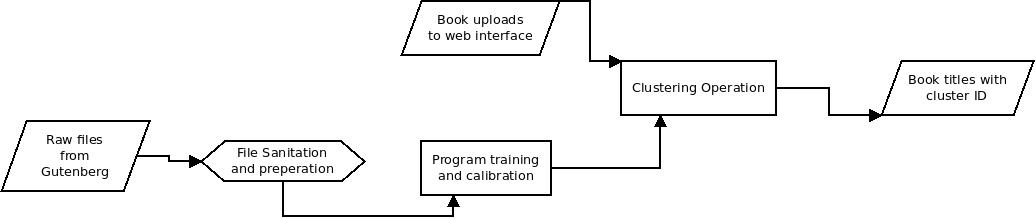
\includegraphics[width=\paperwidth]{../Flowchart.jpg}}
\end{figure}

\begin{figure}
	\label{boxchart}
	\caption{Box diagram of intra-program modules}
	\centering
	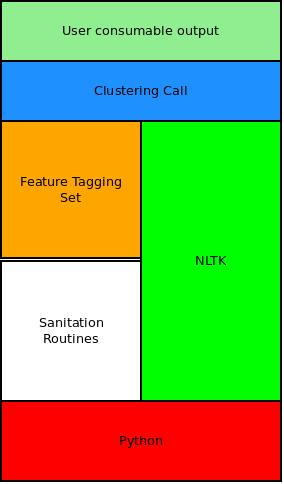
\includegraphics{../StackDiagram.jpg}
\end{figure}

\printbibliography

\end{document}
